\section{Real-time implementation}
\label{sec:rt}

The application consists of two components:
the first handles importing static GTFS data and constructing the network,
while the second implements the \rt models and prediction.
We chose \verb+Rcpp+ to develop the program,
which provides access to other R packages for data manipulation 
(notably \verb+RSQLite+ and \verb+dplyr+),
as well as the speed and memory management capabilities of \verb|C++|. 
The program is implemented in the R package
\verb+transitr+, available on Github (\url{https://github.com/tmelliott/transitr}).
In this section, we discuss the features of the \rt component
and assess its performance in \rt,
both with respect to timing and parameter estimation.

The general structure of the \rt component is shown below,
with the bold steps being those discussed in this paper.
\begin{enumerate}
\item Load GTFS data from database
\item Each time new data are received \ldots
\begin{enumerate}
    \item Update or create new vehicle objects from the new data
    \item \textbf{Run particle filter on each vehicle to update or initialise state}
    \item \textbf{Update state of any roads for which vehicles 
        have completed travel}
    \item Generate ETAs for vehicles using combination of particle filter and network state
    \item Write ETAs to extended Google Protobuf binary file for distribution
\end{enumerate}
\end{enumerate}


During the development of the application,
we were primarily concerned with ensuring each component of the program
is as efficient as possible,
allowing ETAs to be generated and distributed fast enough to be feasible in real-time,
with a target of 30~seconds or faster at peak time.
Using C++ provides the memory management control necessary to make the application
viable in real-time.
We also make use of OpenMP for parallelisation,
since each vehicle is modelled independently so it is trivial to scale up without
worrying about thread safety.


The number of particles needed per vehicle 
depends on many factors,
so it is necessary to explore the performance of the application
with varying number of particles.
Application performance is also assessed
for a range of fixed model parameter values,
such as system noise and GPS error.
To enable comparisons, we implemented a simulated \rt environment
in which the same subset of real vehicle data from 8~October, 2018
could be analysed using a range of settings.
These simulations were carried out of a Virtual Machine 
with 8~cores and 32~Gb of memory, 
running Ubuntu~16.04 and using R~3.4.1.


\subsection{Program Timings}
\label{sec:timings}

In each iteration, 
the timing of the various program components is recorded.
Since the number of vehicles travelling at any given time changes throughout the day,
we used the average timings over an off-peak 15~minute window.
Figure~\ref{fig:timings} shows the average timings for 
varying numbers of particles, $N$.


The most time consuming component is ETA writing,
which involves summarising the individual ETAs estimated for each particle.
While not discussed here this involves quantiles which use a sorting algorithm,
which has complexity $O(N \log N)$ 
which explains the slightly quadratic trend in the timings.


The next most intensive step is vehicle updating,
and takes about 5~seconds for 8000 particles.
The ETA prediction step only takes a few seconds,
although this may increase once a more comprehensive model is developed.
On our 8-core virtual machine the entire process is completed within 20~seconds
when 8000~particles are used.
In the next section we explore the effect of changing $N$
to allow finding the optimal number.


\begin{figure}[tb]
    \centering
    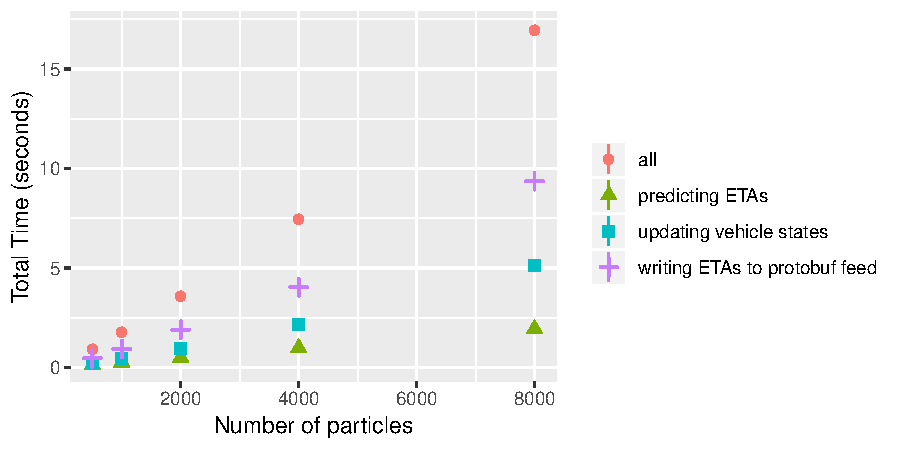
\includegraphics[width=0.7\textwidth]{figures/04_model_results_timing.pdf}
    \caption{
        Application timings were recorded for each component of each
        iteration, and averages over a 15~minute window are shown here.
        The timings shown are \emph{wall time}, the actual time passed,
        not CPU time which would be approximately 8~times larger 
        (for using 8~cores).
        Steps that only involve particle calculations are approximately
        of complexity $O(N)$,
        however some steps are a little more complex, 
        so there is a slightly exponential trend.
    }
        % The timings for various parts of the application, and overall. %
        % The trend is slightly non-linear due to the complexity of the ETA generation step, %
        % which requires sorting of the particle ETAs to obtain quantile estimates.}
    \label{fig:timings}
\end{figure}




\subsection{Model performance}
\label{sec:model_perf}


To evaluate the performance of the model,
the simulation was run using a range of values of GPS error, $\epsilon$,
and system noise, $\sigma^2$.
Figure \ref{fig:dist_to_route} shows the distribution of the distance
between each observation and the route using a nearest point algorithm,
so we chose to use GPS error values $\epsilon \in \{1,2,3,5\}$. 
For the system noise we use values of $\sigma^2\in \{1e^{-4},1e^{-3},1e^{-2},0.05\}$,
which correspond to the average vehicle speed having a variance between 0.1 and 45~meters per second
over a period of 30~seconds.
For each of the combination of these parameter values, along with varying $N$,
several values were computed.
These were effective sample size, $N_\text{eff}$ calculated using (\ref{eq:neff});
degeneration rate, the percentage of iterations in which the vehicle was lost
(no plausible particles);
and the variance of segment travel time estimates.


\begin{figure}[tb]
    \centering
    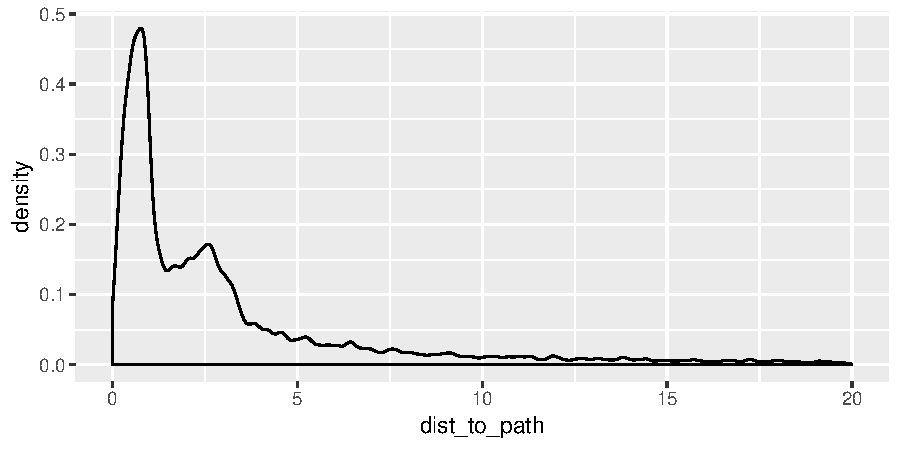
\includegraphics[width=0.7\textwidth]{figures/04_model_results_dist.pdf}
    \caption{
        The distance between the observation and the nearest point on the shape
        is calculated by finding the shortest distance between point and path.
        This gives an approximate idea of GPS error, however it should be noted
        that many observations are made automatically at way points,
        which accounts for the peak at 1m.
        Note also that these observations have been truncated at 20m.
    }
    \label{fig:dist_to_route}
\end{figure}


From Figure~\ref{fig:degen_rate}, we see that $N_\text{eff}$ increases
with GPS error and decreases with system noise.
The degeneration rate decreases with GPS error and increases with $N$,
but is relatively unaffected by system noise.
Large GPS error affects the likelihood,
and gives more weight to particles farther from the observation
than does a smaller GPS error.
Conversely, increasing system noise spreads out the particle cloud,
so fewer particles will be near the vehicle.
Thus, these results are not surprising, 
but show that the model is working as expected.


\begin{figure}[tb]
    \centering
    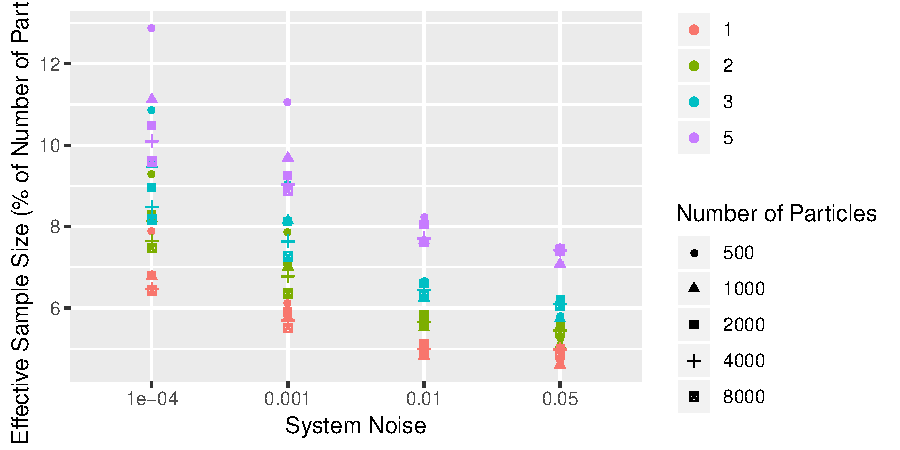
\includegraphics[width=0.9\textwidth]{figures/04_model_results_neff.pdf}
    \caption{
        The effective sample size is an approximate measure of the variance
        of the particle weights.
        When all particles have equal weights, $N_\text{eff} = N$,
        while if all the weight is on one particle, $N_\text{eff} = 1$. 
        The figure is subset by system noise, which shows how $N_\text{eff}$ 
        decreases as system noise increases,
        while increasing GPS error (on the $x$-axis) increases $N_\text{eff}$.
        Increasing $N$ has a negative effect on $N_\text{eff}$ but this is
        only evident when $N_\text{eff}$ is larger.
        The error bars show $\pm 2$SE.
    }
    \label{fig:neff}
\end{figure}

\begin{figure}[tb]
    \centering
    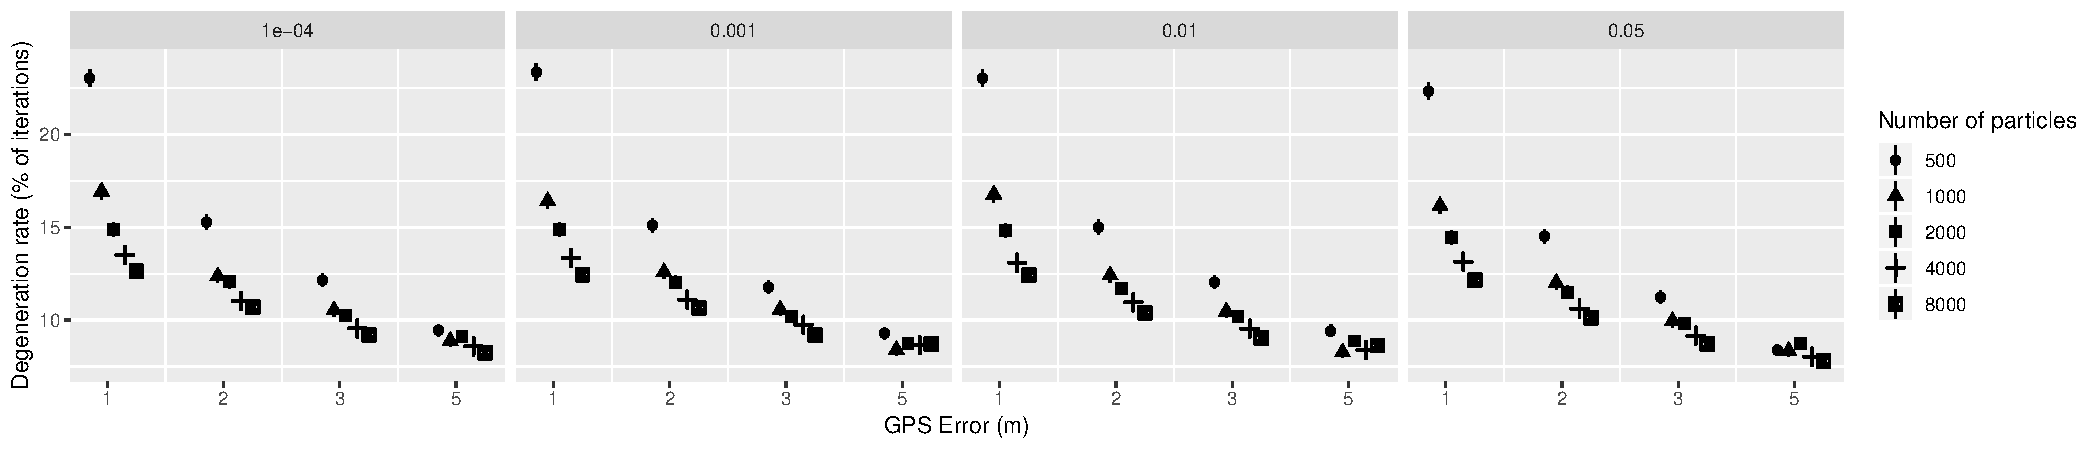
\includegraphics[width=0.9\textwidth]{figures/04_model_results_degen.pdf}
    \caption{
        The degeneration rate is the percentage of iterations where there were no
        plausible particles, so the vehicle was ``lost'' by the model.
        This decreases as GPS error and number of particles increase,
        but there is no visible effect of system noise.
        The error bars show $\pm 2$SE.
    }
    \label{fig:degen_rate}
\end{figure}


The last measure of performance is the relative variance of segment travel times.
This is calculated by computing the average variance of travel times over all simulations,
and then for each simulation, 
taking the average (over road segments) of the ratio between variance for that simulations
and variance for all simulations.
Figure~\ref{fig:travel_times} shows that simulations with larger GPS error
result in a higher relative variance,
while simulations with more particles have lower relative variance.
There is no visible effect of system noise on travel time variation.


The results of the simulations
demonstrate a tradeoff between particle filter performance
($N_\text{eff}$ and degeneration rate) and parameter estimation.
However, until the arrival time prediction model has been completed,
it is difficult to make decisions about the optimal values to use:
we are unable to say whether a higher variation of travel time estimates
is going to have a significant effect on the final ETAs,
particularly when compared to the uncertainty of forecasting road state.


\begin{figure}[tb]
    \centering
    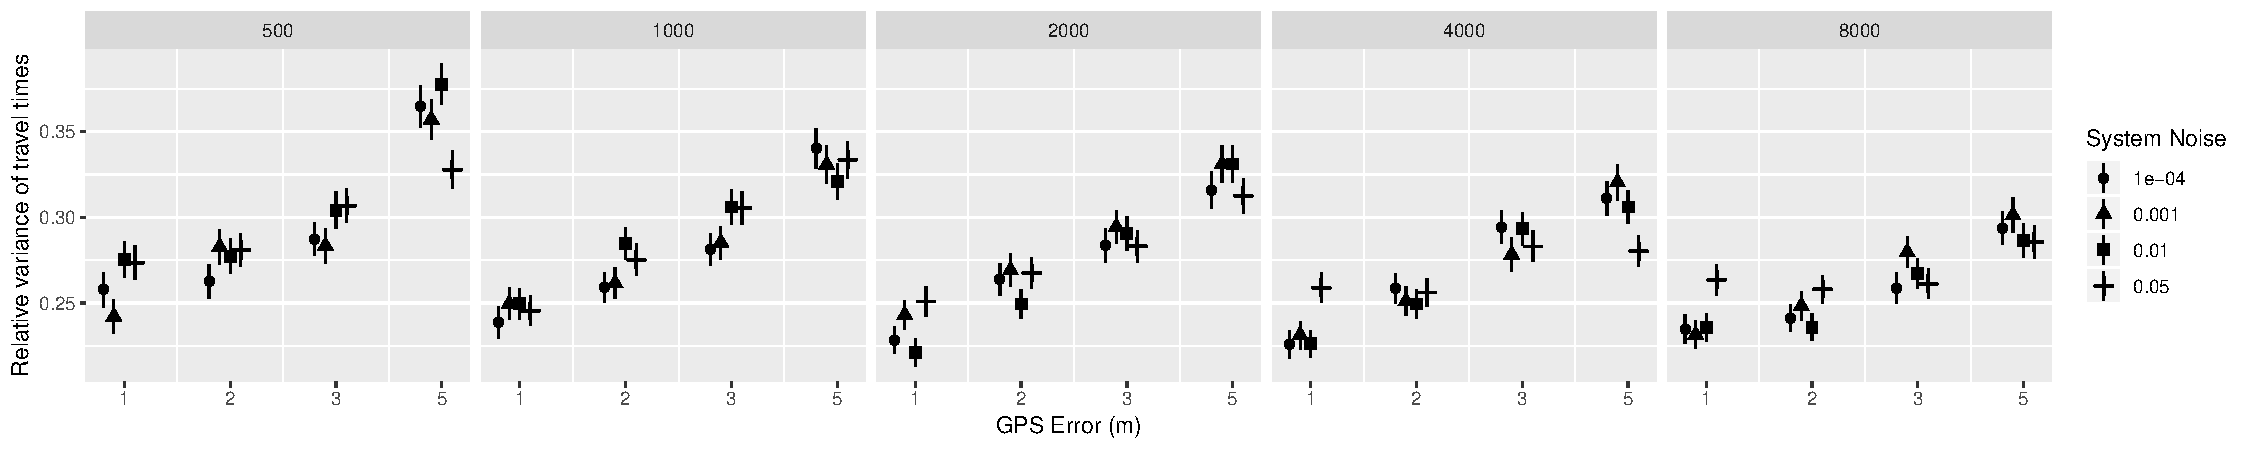
\includegraphics[width=\textwidth]{figures/04_model_results_times.pdf}
    \caption{
        The variability of travel time within a segment increases with GPS error,
        and decreases slightly with increasing number of particles.
        There is no visible effect of system noise on travel time variability.
        The error bars show $\pm 2$SE.
    }
    \label{fig:travel_times}
\end{figure}


